\section{How to start}

Als erstes muss man das Raspberry Pi an einen Bildschirm und an die Stromversorgung anschließen. Hat man alles richtig angeschlossen sollte dieses Bild erscheinen:
\begin{figure}[H]
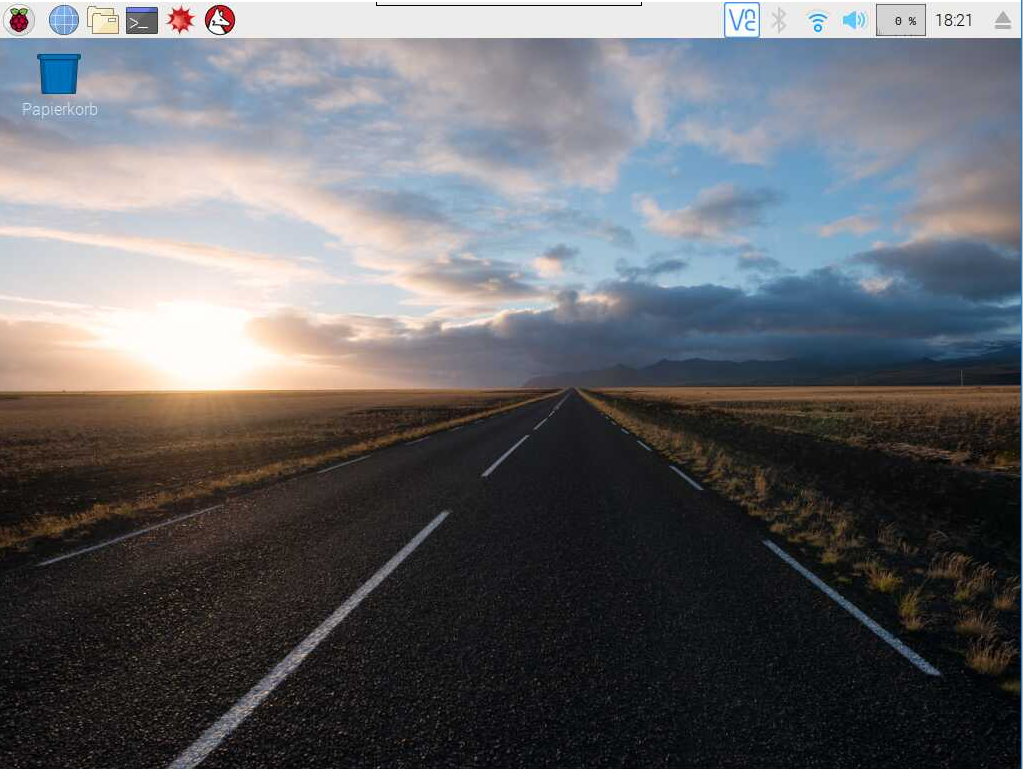
\includegraphics[width=0.5\textwidth]{Bilder/Raspi_Start_Bildschirm.png} %60% der Textbreite
\end{figure}
Als nächstes wird Mincraft Pi gestartet hierzu klickt man wie im nächsten Bild dargestellt auf Mincraft Pi.
\begin{figure}[H]
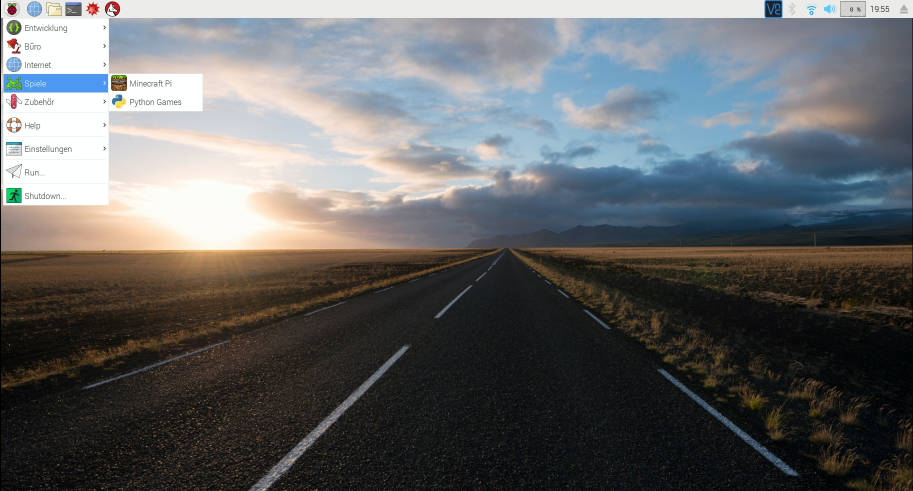
\includegraphics[width=0.5\textwidth]{Bilder/Raspi_Mincraft_Start.png} %60% der Textbreite
\end{figure}
Sobald sich Mincraft Pi geöffnet hat geht man auf "Start Game" $\rightarrowtail$ "Create new". Nun sollte sich das Spiel vollständig gestartet haben - Glückwunsch nun kann Programmiert werden.